%\documentclass[useAMS,usenatbib]{mn2e}
%\bibliographystyle{mn2e}

\documentclass[a4paper,11pt]{article}
%\pdfoutput=1
%\pdfminorversion=5

\usepackage{jcappub}
%\usepackage{widetext}
\usepackage{graphicx}
%\usepackage{dcolumn}
\usepackage{bm}
\usepackage{amssymb,amsmath,bm,dsfont}
\usepackage{color}
\usepackage[dvipsnames]{xcolor}
%\usepackage[colorlinks,linkcolor=red,citecolor=blue,urlcolor=blue ]{hyperref}
%\usepackage{multirow}
\usepackage[utf8]{inputenc}
\usepackage{balance}
\usepackage{enumitem}
\usepackage{lipsum}
\usepackage[caption=false]{subfig}

\newcommand{\nv}{\hat{\mathbf{\theta}}}
\newcommand{\kalo}{Karhunen-Lo\`{e}ve~}
\newcommand{\cfh}{CFHTLenS~}
\newcommand{\jcap}{JCAP}
\newcommand{\mnras}{MNRAS}
\newcommand{\aap}{A\&A}
\newcommand{\aaps}{A\&AS}
\newcommand{\apjs}{ApJS}
\newcommand{\apj}{ApJ}
\newcommand{\apjl}{ApJL}
\newcommand{\prd}{Phys.~Rev.~D}
\newcommand{\prl}{Phys.~Rev.~Lett.}
\newcommand{\aj}{Astron. Journal}
\newcommand{\pasp}{Publications of the ASP}
\newcommand{\nar}{New Astronomy Review}
\newcommand{\procspie}{Proceedings of the SPIE}
\newcommand{\physrep}{Physics Reports}

\newcommand{\todo}[1]{{\bf TODO: #1}}
%\newcommand{\todo}[1]{$\,$}

\newcommand{\PCL}{pseudo-$C_\ell$~}
\newcommand{\pcl}[3]{\hat C_{#1}^{#2 #3}}
\newcommand{\avg}[1]{\langle #1 \rangle}
\newcommand{\fsky}{f_{\mbox{\rm sky}}}
\newcommand{\clth}{C_\ell^{th}}
\newcommand{\clc}{C_\ell^{cont}}
\newcommand{\cl}{C_\ell}
\newcommand{\summ}[1]{\sum_{\bf #1}\Delta #1^2}
\newcommand{\Ylm}[3]{{\sf E}^{#1}_{\bf #2}({\bf #3})}
\newcommand{\red}[1]{{\color{red} #1}}
\newcommand{\wtj}[6]{\left(\begin{array}{ccc} #1 & #2 & #3\\#4 & #5 & #6\end{array} \right)}
\newcommand{\lbpw}{\ell_{\mbox{bpw}}}

%\title[Disconnected pseudo-$C_\ell$ covariances for projected datasets]{Disconnected pseudo-$C_\ell$ covariances for projected datasets}
\title{\boldmath Disconnected pseudo-$C_\ell$ covariances for projected datasets}

\author[a]{Carlos Garc\'{i}a-Garc\'{i}a}
\author[b]{David Alonso}
\author[b]{Emilio Bellini}

\affiliation[a]{Instituto de Física Fundamental, Consejo Superior de Investigaciones Científicas, c/. Serrano 123, E–28006, Madrid, Spain}
\affiliation[b]{Oxford Astrophysics, Department of Physics, Keble Road, Oxford, OX1 3RH, UK}

\emailAdd{carlosgarcia@iff.csic.es}
\emailAdd{david.alonso@physics.ox.ac.uk}
\emailAdd{emilio.bellini@physics.ox.ac.uk}

\abstract{\lipsum[1]}

\begin{document}
  \maketitle
  \flushbottom

  \section{Introduction}\label{sec:intro}
    The two-point correlation of different fields projected on the celestial sphere is one of the most common observables used in the analysis of large datasets in astrophysics, from studies of the Cosmic Microwave Background \todo{cites} to large-scale structure and weak lensing surveys \todo{cites}. Using these two-point functions achieves a high level of data compression (with respect to the size of the raw datasets -- time-ordered data, images or catalogs), and they can be directly used to constrain cosmological and astrophysical parameters assuming that one can model their likelihood. This is usually done by assuming that the two-point functions are Gaussianly distributed, which is often good approximation due to the central limit theorem \todo{cites}. In this case, the only obstacle that remains is being able to estimate the covariance matrix of a set of two-point correlators. Since the form of this covariance directly affects the posterior parameter uncertainties, a precise determination of it is of paramount importance. In large-scale structure experiments this has often been resolved by making use of one's own data through resampling techniques \todo{cites}, or by generating a large number of mock realizations \todo{cites}. With the advent of the larger current and future surveys, the increasing size of the data vector and of the volume to be simulated has made this solution impractical, and fully analytical and hybrid estimators are now being used.
  
    The problem of producing accurate analytical estimates of the covariance matrix for large-scale structure data has seen significant progress in the last few years \todo{cite}. As described in \todo{cite}, the covariance matrix recieves three main contributions:
    \begin{itemize}
      \item {\bf Gaussian covariance:} this is the contribution to the covariance from the disconnected part of the trispectrum of the different fields involved (also called the ``disconnected'' covariance). In simpler terms, this is the covariance matrix one would obtain if all fields involved were Gaussianly distributed.
      \item {\bf Connected non-Gaussian covariance:} this is the contribution from the connected trispectrum (which would vanish if all fields were Gaussianly distributed.
      \item {\bf Super-sample covariance:} this is the additional coupling between different scales induced by density fluctuations on scales larger than the volume mapped.
    \end{itemize}
  
    On most scales relevant for cosmological studies, the Gaussian contribution dominates the error budget, although the connected and super-sample terms cannot be neglected \todo{cite}. The Gaussian contribution is trivial to compute for fields observed over the full sky:
    \begin{equation}
      {\rm Cov}\left(C^{ab}_\ell,C^{cd}_\ell\right)=\delta^K_{\ell\ell'}\frac{C^{ac}_\ell C^{bd}_\ell+C^{ad}_\ell C^{bc}_\ell}{2\ell+1},
    \end{equation}
    where $C^{xy}_\ell$ is the angular power spectrum between two maps $x$ and $y$ on multipole $\ell$. Unfortunately, the presence of a sky mask in general induces non-trivial couplings between different $\ell$s, which must be accurately estimated in order to produce unbiased evaluations of the parameter likelihood \todo{cite}.
  
    In this paper we will present and generalise methods developed in the context of CMB experiments to account for the impact of survey geometry on the Gaussian part of the power spectrum covariance matrix \todo{cites}, and will study in detail the performance of these methods for large-scale structure and weak lensing datasets. We have also implemented these approximations in the public code {\tt NaMaster}, making the computation of accurate Gaussian covariance matrices significantly simpler.

    The paper is structured as follows: Section \ref{sec:theory} presents the methods and approximations used to calculate accurate covariances. In Section \ref{sec:results} we test the methods against Gaussian simulations and study their performance as well as their impact on the final cosmological parameter estimation. We then summarize our results and conclude in Section \ref{sec:discussion}. Appendix \ref{app:flat} presents the performance of these methods for flat-sky approximation, and we provide technical details of the software implementation in Appendix \ref{app:namaster}.

  \section{Analytical Gaussian covariances}\label{sec:theory}
    \subsection{Preliminaries}\label{ssec:theory.prelim}
      \todo{cites everywhere}
      We will deal with spin-0 and spin-2 fields defined on a 2-dimensional space. We will use a generic notation that can then be applied to both curved and flat skies. Given a field ${\bf a}({\bf x})$, with 1 (spin-0) or 2 components (spin-2), and defined on the coordinates ${\bf x}$, we define its generalized Fourier coefficients as
      \begin{equation}
        {\bf a}_{\bf k}=\summ{x}\,\Ylm{\dag}{k}{x}\,{\bf a}({\bf x}),
      \end{equation}
      where the operator $\summ{x}$ denotes a integral or sum of all coordinates ${\bf x}$, and $\Ylm{\dag}{k}{x}$ are a set of orthogonal functions. We will also assume that the $\Ylm{\dag}{k}{x}$ are a \emph{complete} set of basis functions, in which case:
      \begin{align}
        &\summ{x}\,\Ylm{\dag}{k}{x}\Ylm{}{l}{x}=\mathds{1}\Delta^x({\bf k},{\bf l}),\\
        &\summ{k}\,\Ylm{}{k}{x}\Ylm{\dag}{k}{y}=\mathds{1}\Delta^k({\bf x},{\bf y}),
      \end{align}
      where $\summ{k}$ denotes an integral over all possible generalised Fourier coefficients ${\bf k}$, and $\Delta^x$ and $\Delta^k$ are generalized delta functions:
      \begin{align}
        &\summ{k}\,f({\bf k})\Delta^x({\bf k},{\bf l})\equiv f({\bf l}),\\
        &\summ{x}\,f({\bf x})\Delta^k({\bf x},{\bf y})\equiv f({\bf y}).
      \end{align}
      For a spin-$s$ quantity, $\Ylm{}{l}{x}$ can be written in terms of two spin-raising and spin-lowering operators, $\eth$ and $\bar{\eth}$, and a set of scalar orthogonal functions $q({\bf l},{\bf x})$ as:
      \begin{equation}
        \Ylm{}{l}{x}=-\frac{\beta_{\ell,s}}{2}\left(
        \begin{array}{cc}
          \eth^s+\bar{\eth}^s & i(\eth^s-\bar{\eth}^s)\\
          -i(\eth^s-\bar{\eth}^s) & \eth^s+\bar{\eth}^s
        \end{array}\right) q({\bf l},{\bf x}),
      \end{equation}
      where $\beta_{\ell,s}$ is a normalization factor defined in Table \ref{tab:notation}.
    
      Finally, we will assume that all fields are Gaussian stochastic fields that are additionally statistically isotropic. As a consequence of this, different generalised Fourier modes are uncorrelated:
      \begin{equation}\label{eq:iso}
        \langle {\bf a}_{\bf k}{\bf b}^\dag_{\bf l}\rangle\equiv {\sf C}^{ab}_\ell\,K\,\Delta^x({\bf k},{\bf l}),
      \end{equation}
      where $K$ is a volume factor (see below) and ${\sf C}^{ab}_k$ is the power spectrum. Defined this way, the power spectrum is a matrix, with elements
      \begin{equation}
        \left\langle a^\alpha_{\bf k}\left(b^\beta_{\bf l}\right)^*\right\rangle\equiv \left({\sf C}^{ab}_\ell\right)_{\alpha\beta}\,K\,\Delta^x({\bf k},{\bf l}),
      \end{equation}
      where $a^\alpha$ is the $\alpha$-th element of field ${\bf a}$. It will often be useful in what follows to think of ${\sf C}^{ab}_\ell$ as a 1-dimensional vector that we will denote by ${\rm vec}({\sf C}^{ab}_\ell)$. To do so, we simply map the two indices $(\alpha,\beta)$ into a single number $A$, such that ${\rm vec}({\sf C}^{ab}_\ell)_A = ({\sf C}^{ab}_\ell)_{\alpha\beta}$.
    
      \begin{table*}
        \centering
        \begin{tabular}{|c|c|c|}
          \hline
          Symbol & Curved sky & Flat sky (continuum $\rightarrow$ discretized) \\
          \hline
          \(\displaystyle {\bf l} \) & \(\displaystyle (\ell,m) \) & \(\displaystyle (l_x,l_y) \) \\
          \(\displaystyle \summ{l} \) & \(\displaystyle \sum_{\ell=0}^{\infty} \sum_{m=-\ell}^{\ell} \) & \(\displaystyle \int \frac{dl^2}{2\pi} \rightarrow \sum_{\bf l}\frac{2\pi}{L_xL_y}\) \\
          \(\displaystyle \Delta^x({\bf l},{\bf l}')\) & \(\displaystyle \delta^K_{\ell\ell'}\delta^K_{mm'}\) & \(\displaystyle 2\pi\,\delta^D({\bf l}-{\bf l}')\rightarrow \delta^K_{l_xl'_x}\delta^K_{l_yl'_y}\frac{L_xL_y}{(2\pi)^2}2\pi\) \\
          \(\displaystyle {\bf x}\) & \(\displaystyle \nv\equiv(\theta,\varphi) \) & \(\displaystyle (x,y)\) \\
          \(\displaystyle \summ{x} \) & \(\displaystyle \int_0^{\phi} d\phi \int_{-1}^{1} d(\cos\theta)\) & \(\displaystyle \int \frac{dx^2}{2\pi}\rightarrow\sum_{\bf x}\frac{L_xL_y}{2\pi N_xN_y}\) \\
          \(\displaystyle \Delta^k({\bf x},{\bf y})\) & \(\displaystyle \delta^D(\cos\theta-\cos\theta')\delta^D(\varphi-\varphi')\) & \(\displaystyle 2\pi\,\delta^D({\bf x}-{\bf y})\rightarrow\delta^K_{xx'}\delta^K_{yy'}\frac{N_xN_y}{L_xL_y}2\pi\) \\
          \(\displaystyle q({\bf l},{\bf x})\) & \(\displaystyle Y_{\ell m}(\nv)\) & \(\displaystyle e^{i{\bf l}\cdot{\bf x}}\) \\
          \(\displaystyle \eth\,_sf\) & \(\displaystyle -(\sin\theta)^s\left(\partial_\theta+i\frac{\partial_\varphi}{\sin\theta}\right)(\sin\theta)^{-s}\,_sf(\nv)\) & \(\displaystyle (\partial_x-i\partial_y)\,_sf\) \\
          \(\displaystyle \bar{\eth}\,_sf\) & \(\displaystyle -(\sin\theta)^{-s}\left(\partial_\theta-i\frac{\partial_\varphi}{\sin\theta}\right)(\sin\theta)^s\,_sf(\nv)\) & \(\displaystyle (\partial_x+i\partial_y)\,_sf\) \\
          \(\displaystyle \beta_{\ell,s}\) & \(\displaystyle \sqrt{\frac{(\ell-2)!}{(\ell+2)!}}\) & \(\displaystyle \ell^{-s}\) \\
          \(\displaystyle K \) & \(\displaystyle 1 \) & \(\displaystyle (2\pi)^{-1}\) \\
          \hline
        \end{tabular}
        \caption{Lookup table describing the generalized notation introduced in Section \ref{ssec:theory.prelim} for quantities defined on the sphere (second column) and on the flat 2D plane (third column). For the flat-sky case, we also provide expressions for a discretized, finite 2D plane with periodic boundary conditions. In this case, the map has dimensions $(L_x,L_y)$ subdivided into $(N_x,N_y)$ equi-spaced pixels in $(x,y)$. $\delta^D$ and $\delta^K$ are the Dirac and Kronecker delta functions respectively.}\label{tab:notation}
      \end{table*}

      All the functions and operators above can be specialised to fields defined on the sphere or the 2D plane (flat sky approximation) as described in Table \ref{tab:notation}.

    \subsection{The pseudo-$C_\ell$ method}\label{ssec:theory.pcl}
      This section provides a very brief introduction to the \PCL power spectrum estimator. Further details can be found in \todo{cite}. 
      In any practical situation we do not have access to maps of a given field ${\bf a}$ over the full sky, but rather to a weighted or masked version of them
      \begin{equation}
        \tilde{\bf a}({\bf x})\equiv w_a({\bf x}){\bf a}({\bf x}),
        \label{eq:mask}
      \end{equation}
      where $w_a$ is commonly called the ``mask''. Due to the convolution theorem, the generalized Fourier coefficients of the masked field will be a convolution of the mask and true field coefficients:
      \begin{align}\nonumber
        \tilde{\bf a}_{\bf l}=&\summ{k}\left[\summ{x}\,w^a({\bf x})\,\Ylm{\dag}{l}{x}\,\Ylm{}{k}{x}\right]{\bf a}_{\bf k}\\
                        \equiv&\summ{l}\,^a{\sf M}_{{\bf l}{\bf k}}\,{\bf a}_{\bf k},
      \end{align}
      where we have defined the mode-coupling coefficients $\,^a{\sf M}_{{\bf l}{\bf k}}$ in the second line.
    
      Correlating the generalized Fourier coefficients of two masked fields therefore yields a mode-coupled version of their true underlying power spectrum:
      \begin{align}\nonumber
        \left\langle\tilde{\bf a}_{\bf l}\tilde{\bf b}^\dag_{\bf l}\right\rangle=&\summ{k}\summ{q}\,^a{\sf M}_{{\bf l}{\bf k}}\left\langle{\bf a}_{\bf k}{\bf b}^\dag_{\bf q}\right\rangle\,^b{\sf M}^\dag_{{\bf l}{\bf q}}\\
                                                                              =&K\,\summ{k}\,^a{\sf M}_{{\bf l}{\bf k}}{\sf C}^{ab}_k\,^b{\sf M}^\dag_{{\bf l}{\bf k}} \label{eq:M}                                                                             
      \end{align}
    
      The \PCL estimator then proceeds in two steps:
      \begin{enumerate}
        \item We first bin different ${\bf l}$ modes into sets of them called bandpowers (typically bands of similar $\ell$ or annuli of flat-sky Fourier modes spanning a narrow range of radii). Let us denote a given bandpower by its index $q$. The binned pseudo-power spectrum is:
        \begin{equation}
          \tilde{\sf C}^{ab}_q=\sum_{{\bf l}\in q} B_q^{\bf l}\,\tilde{\bf a}_{\bf l}\tilde{\bf b}^\dag_{\bf l},
        \end{equation}
        where the bandpower weights are normalized such that $\sum_{{\bf l}\in q}B_q^{\bf l}=(K\Delta^x({\bf l},{\bf l}))^{-1}$.
        \item Then, the correlation between bandpowers induced by the mode-coupling coefficients is partially reversed by multiplying $\tilde{\sf C}^{ab}_q$ by the so-called binned ``mode-coupling matrix'' $\mathcal{M}$, giving the final estimator
        \begin{equation}
          {\rm vec}\left(\hat{\sf C}^{ab}_q\right) = \sum_{q'} \left(\mathcal{M}^{-1}\right)_{qq'}\,{\rm vec}\left(\tilde{\sf C}^{ab}_{q'}\right).
        \end{equation}

        The main advantage of the \PCL estimator is that the mode-coupling matrix $\mathcal{M}$ is directly related to the coupling coefficients $\,^a{\sf M}_{{\bf l}{\bf l}'}$ (see \todo{cite}), and can be computed analytically making use of methods that scale like $\ell_{\rm max}^3$.
      \end{enumerate}
    
      For completeness, the mode-coupling matrices for flat-sky and curved-sky fields are given by \todo{cite}:
      \begin{itemize}
        \item {\bf Curved sky.} After averaging over the harmonic number $m$, the mode-coupling matrices are:
        \begin{equation}
          \left\langle\frac{1}{2\ell+1}\sum_{m=-\ell}^\ell {\rm vec}\left[\tilde{\bf a}_{\bf l}\tilde{\bf b}^\dag_{\bf l}\right]\right\rangle=\sum_{\ell'}{\sf M}^{s_as_b}_{\ell\ell'} {\rm vec}\left[{\sf C}^{ab}_{\ell'}\right],
        \end{equation}
        with
        \begin{align}
          &{\sf M}^{00}_{\ell\ell'}=(2\ell'+1)\,\Xi^{00}_{\ell\ell'}(w_a,w_b),\hspace{12pt}
          {\sf M}^{02}_{\ell\ell'}=(2\ell'+1)\,\Xi^{0+}_{\ell\ell'}(w_a,w_b)\,\mathds{1},\\
          &{\sf M}^{22}_{\ell\ell'}=(2\ell'+1)
          \left(
          \begin{array}{cccc}
            \Xi^{++}_{\ell\ell'} & 0 & 0 & \Xi^{--}_{\ell\ell'} \\
            0 & \Xi^{++}_{\ell\ell'} & -\Xi^{--}_{\ell\ell'} & 0 \\
            0 & -\Xi^{--}_{\ell\ell'} & \Xi^{++}_{\ell\ell'} & 0 \\
            \Xi^{--}_{\ell\ell'} & 0 & 0 & \Xi^{++}_{\ell\ell'}
          \end{array}\right),\\\nonumber
        \end{align}
        where
        \begin{align}\label{eq:coeff_mcm}
          &\Xi^{00}_{\ell\ell'}(w,v)  \equiv\sum_{\ell''}\frac{P^{wv}_{\ell''}}{4\pi}\wtj{\ell}{\ell'}{\ell''}{0}{0}{0}^2\\
          &\Xi^{0+}_{\ell\ell'}(w,v)  \equiv\sum_{\ell''}\frac{P^{wv}_{\ell''}}{4\pi}\wtj{\ell}{\ell'}{\ell''}{0}{0}{0}\wtj{\ell}{\ell'}{\ell''}{2}{-2}{0}\\
          &\Xi^{\pm\pm}_{\ell\ell'}(w,v) \equiv\sum_{\ell''}\frac{P^{wv}_{\ell''}}{4\pi}\wtj{\ell}{\ell'}{\ell''}{2}{-2}{0}^2\frac{1\pm(-1)^{\ell+\ell'+\ell''}}{2}.
        \end{align}
        Here the 2-by-3 matrix-like quantities are the Wigner 3-$j$ symbols, and
        \begin{equation}
          P^{vw}_\ell\equiv\sum_{m=-\ell}^\ell v_{\ell m}w^*_{\ell m}.
        \end{equation}
        \item {\bf Flat sky.} In this case the averaging over the Fourier-space azimuth happens while binning into bandpowers, and therefore the unbinned mode-coupling matrix is defined before binning. Assuming flat bandpowers, such that $B_q^{\bf l}=(2\pi)^2/(L_xL_yN_q)$, where $N_q$ is the number of Fourier-space modes in the $q$-th bandpower:
        \begin{equation}
          \left\langle{\rm vec}\left[\tilde{\sf C}^{ab}_q\right]\right\rangle=\sum_{{\bf l}\in q}\frac{1}{N_q} \sum_{\bf k}{\sf M}^{s_as_b}_{{\bf l}{\bf k}}\,{\rm vec}\left[{\sf C}^{ab}_k\right]
        \end{equation}
        with
        \begin{align}
          {\sf M}^{00}_{{\bf l}\,{\bf k}}&\equiv \bar{\Xi}^{00}_{{\bf l}{\bf k}},\\\label{eq:m02_flat}
          {\sf M}^{02}_{{\bf l}\,{\bf k}}&\equiv 
          \left(
          \begin{array}{cc}
            \bar{\Xi}^{0+}_{{\bf l}{\bf k}} & -\bar{\Xi}^{0-}_{{\bf l}{\bf k}} \\
            \bar{\Xi}^{0-}_{{\bf l}{\bf k}} &  \bar{\Xi}^{0+}_{{\bf l}{\bf k}}
          \end{array}\right)\\\label{eq:m22_flat}
          {\sf M}^{22}_{{\bf l}\,{\bf k}}&\equiv 
          \left(
          \begin{array}{cccc}
            \bar{\Xi}^{++}_{{\bf l}{\bf k}} & -\bar{\Xi}^{+-}_{{\bf l}{\bf k}} & -\bar{\Xi}^{+-}_{{\bf l}{\bf k}} &  \bar{\Xi}^{--}_{{\bf l}{\bf k}} \\
            \bar{\Xi}^{+-}_{{\bf l}{\bf k}} &  \bar{\Xi}^{++}_{{\bf l}{\bf k}} & -\bar{\Xi}^{--}_{{\bf l}{\bf k}} & -\bar{\Xi}^{+-}_{{\bf l}{\bf k}} \\
            \bar{\Xi}^{+-}_{{\bf l}{\bf k}} & -\bar{\Xi}^{--}_{{\bf l}{\bf k}} &  \bar{\Xi}^{++}_{{\bf l}{\bf k}} & -\bar{\Xi}^{+-}_{{\bf l}{\bf k}} \\
            \bar{\Xi}^{--}_{{\bf l}{\bf k}} &  \bar{\Xi}^{+-}_{{\bf l}{\bf k}} &  \bar{\Xi}^{+-}_{{\bf l}{\bf k}} & \bar{\Xi}^{++}_{{\bf l}{\bf k}}
          \end{array}\right),
        \end{align}
        where
        \begin{align}
          &\bar{\Xi}^{00}_{{\bf l}{\bf k}}=\left(\frac{2\pi}{L_xL_y}\right)^2 (w_a)_{{\bf l}-{\bf k}}(w_b)^*_{{\bf l}-{\bf k}},\\
          &\bar{\Xi}^{0+}_{{\bf l}{\bf k}}=\left(\frac{2\pi}{L_xL_y}\right)^2 (w_a)_{{\bf l}-{\bf k}}(w_b)^*_{{\bf l}-{\bf k}}\cos2\Delta\varphi,\\
          &\bar{\Xi}^{0-}_{{\bf l}{\bf k}}=\left(\frac{2\pi}{L_xL_y}\right)^2 (w_a)_{{\bf l}-{\bf k}}(w_b)^*_{{\bf l}-{\bf k}}\sin2\Delta\varphi,\\
          &\bar{\Xi}^{++}_{{\bf l}{\bf k}}=\left(\frac{2\pi}{L_xL_y}\right)^2 (w_a)_{{\bf l}-{\bf k}}(w_b)^*_{{\bf l}-{\bf k}}\cos^22\Delta\varphi,\\
          &\bar{\Xi}^{+-}_{{\bf l}{\bf k}}=\left(\frac{2\pi}{L_xL_y}\right)^2 (w_a)_{{\bf l}-{\bf k}}(w_b)^*_{{\bf l}-{\bf k}}\cos2\Delta\varphi\,\sin2\Delta\varphi,\\
          &\bar{\Xi}^{--}_{{\bf l}{\bf k}}=\left(\frac{2\pi}{L_xL_y}\right)^2 (w_a)_{{\bf l}-{\bf k}}(w_b)^*_{{\bf l}-{\bf k}}\sin^22\Delta\varphi,\\
        \end{align}
        and $\Delta\varphi$ is the relative angle between ${\bf l}$ and ${\bf k}$.
      \end{itemize}

      Before we move on to covariances, it is worth considering the case of unmasked field (i.e $w^a({\bf x})=1$ everywhere). In this case $\,^a{\sf M}_{{\bf l}{\bf l}'}=\mathds{1}\Delta^x({\bf k},{\bf l})$, and therefore different modes are uncorrelated (as should have been obvious). In a non-ideal case where the mask is still sufficiently well behaved (i.e. masks without too much small-scale structure), we can still expect the coupling coefficients $\,^a{\sf M}_{{\bf l}{\bf l}'}$ to be sharply peaked around ${\bf l}={\bf l}'$.
  
    \subsection{Covariance matrices}\label{ssec:theory.pclcov}
      So far we have not assumed anything about the statistics of the fields, other than the fact that they are isotropic (Eq. \ref{eq:iso}). This section presents a method to estimate the disconnected part of the power spectrum covariance for the \PCL estimator, which is the contribution to the power spectrum covariance if all fields involved were Gaussianly distributed.
    
      Let $A$ and $F$ be the vector indices corresponding to the pairs of field indices $(\alpha,\beta)$ and $(\phi,\gamma)$ respectively, and let us start by considering the covariance
      \begin{equation}
        \Sigma^{AF}_{{\bf l}{\bf l}'}\equiv\left\langle\tilde{a}^\alpha_{\bf l}\tilde{b}^{\beta *}_{\bf l}\tilde{f}^\phi_{{\bf l}'}\tilde{g}^{\gamma *}_{{\bf l}'}\right\rangle-\left\langle\tilde{a}^\alpha_{\bf l}\tilde{b}^{\beta *}_{\bf l}\right\rangle\left\langle\tilde{f}^\phi_{{\bf l}'}\tilde{g}^{\gamma *}_{{\bf l}'}\right\rangle
      \end{equation}
      The covariance of the binned bandpowers $\tilde{\sf C}$ can then be computed as
      \begin{equation}\label{eq:cov_binned}
        {\rm Cov}\left({\rm vec}\left(\tilde{\sf C}^{ab}_q\right)_A,{\rm vec}\left(\tilde{\sf C}^{fg}_{q'}\right)_F\right)=\sum_{{\bf l}\in q} B^{\bf l}_q\sum_{{\bf l}'\in q'} B^{{\bf l}'}_{q'}\,\Sigma^{AF}_{{\bf l}{\bf l}'}.
      \end{equation}
      which can then be used to estimate the covariance of the mode-decoupled bandpowers multiplying it by the inverse mode-coupling matrix twice. I.e., schematically:
      \begin{equation}
        {\rm Cov}\left(\hat{\sf C}\right)=\mathcal{M}^{-1}\cdot{\rm Cov}\left(\tilde{C}\right)\cdot\left(\mathcal{M}^{-1}\right)^{T},
      \end{equation}
      where we have suppressed all indices for simplicity. The problem of estimating the \PCL covariance therefore reduces to estimating $\Sigma^{AC}_{\ell\ell'}$.
    
      We now make use of Wick's theorem, which states that, for Gaussian fields $\langle a\,b\,f\,g\rangle=\langle a\,b\rangle\langle f\,g\rangle+\langle a\,f\rangle\langle b\,g\rangle+\langle a\,g\rangle\langle b\,f\rangle$. In this case, the expression for $\Sigma^{AF}_{{\bf l}{\bf l'}}$ reads:
      \begin{align}\nonumber
        \Sigma^{AF}_{{\bf l}{\bf l}'}=&\left[K\summ{k}\,^aM^{\alpha\alpha'}_{{\bf l}{\bf k}}\,^gM^{\gamma\gamma'*}_{{\bf l}'{\bf k}}C^{ag,(\alpha'\gamma')}_k\right]\left[\summ{q}\,^bM^{\beta\beta'*}_{{\bf l}{\bf q}}\,^fM^{\phi\phi'}_{{\bf l}'{\bf q}}C^{bf,(\beta'\phi')}_q\right]^*\\\label{eq:covar_general}
        &+\left((g,\gamma)\leftrightarrow(f,\phi)\right),
      \end{align}
      where we implicitly sum over repeated indices (e.g. $\alpha'$), and the second term is equivalent to the first one after swapping the roles of fields ${\bf f}$ and ${\bf g}$. Without any further approximations, for each pair $({\bf l},{\bf l}')$, we would need to perform two 2-dimensional integrals, and therefore the calculation would scale like $\ell_{\rm max}^6$, quickly becoming unfeasible.
    
      Under the assumption that the coupling coefficients $M_{{\bf l}{\bf k}}$ are sharply peaked around ${\bf l}={\bf k}$, we can simplify the expression above approximating the power spectra as constants within the support of the coupling coefficients. Explicitly, we approximate 
      \begin{equation}\nonumber
        C^{ag,(\alpha'\gamma')}_kC^{bf,(\beta',\phi')}_q\simeq C^{ag,(\alpha'\gamma')}_{(\ell}C^{bf,(\beta',\phi')}_{\ell')}\equiv\frac{1}{2}\left(C^{ag,(\alpha'\gamma')}_\ell C^{bf,(\beta',\phi')}_{\ell'}+C^{ag,(\alpha'\gamma')}_{\ell'} C^{bf,(\beta',\phi')}_\ell\right).
      \end{equation}
      In this case, the expression for $\Sigma^{AF}_{{\bf l}{\bf l}'}$ simplifies to
      \begin{align}\label{eq:covar_efstathiou}
        \Sigma^{AF}_{{\bf l}{\bf l}'}=C^{ag,(\alpha'\gamma')}_{(\ell}C^{bf,(\beta',\phi')}_{\ell')}\,^{ag}W^{\alpha\gamma,\alpha'\gamma'}_{{\bf l}{\bf l}'}\left(\,^{bf}W^{\beta\phi,\beta'\phi'}_{{\bf l}{\bf l}'}\right)^*+\left((g,\gamma)\leftrightarrow(f,\phi)\right),
      \end{align}
      where we have defined the covariance coupling coefficients
      \begin{equation}\label{eq:covar_coupling}
        \,^{ab}W^{\alpha\beta,\alpha'\beta'}_{{\bf l}{\bf l}'}=\summ{k}\,^aM^{\alpha\alpha'}_{{\bf l}{\bf k}}\left(\,^bM^{\beta\beta'}_{{\bf l}'{\bf k}}\right)^*.
      \end{equation}

      In order to compute these coefficients, let us start by defining the quantities
      \begin{equation}
        \,^{ab}I^{\pm s_a,\pm s_b}_{{\bf l}{\bf l'}}\equiv\summ{k}\summ{x}\summ{y}w_a({\bf x})w_b({\bf y})\,q^{\pm s_a}_{{\bf l}{\bf k}}({\bf x})\,\left(q^{\pm s_b}_{{\bf l}'{\bf k}}({\bf y})\right)^*,
      \end{equation}
      where $s_a$ is the spin of field ${\bf a}$, and
      \begin{equation}
        q^{\pm s}_{{\bf l}{\bf k}}({\bf x})\equiv \frac{\beta_{\ell,s}\beta_{k,s}}{2}\left(\left[\eth^s q({\bf l},{\bf x})\right]^* \eth^sq({\bf k},{\bf x})\pm\left[\bar{\eth}^sq({\bf l},{\bf x})\right]^*\bar{\eth}^sq({\bf k},{\bf x})\right).
      \end{equation}

      Now, in what follows, we will be concerned with the auto- and cross-correlations of spin-0 and spin-2 fields. Thus, to simplify the notation, we will enumerate the different types of coupling coefficients that exist for a spin-0 field with a single component that we will call $\delta$, in analogy to the projected galaxy overensity, and for a spin-2 field $\mathbf{\gamma}$ with $E$ and $B$ components $\gamma_E$ and $\gamma_B$, in analogy to the cosmic shear field. With this setup, all the possible non-zero $W^{\alpha\beta,\alpha'\beta'}_{{\bf l}{\bf l}'}$ can be expressed in terms of the $I^{\pm s_a,\pm s_b}_{{\bf l}{\bf l}'}$ as follows:
      \begin{align}\label{eq:coeff}
        &W^{\delta\delta,\delta\delta}_{{\bf l},{\bf l}'}=I^{0,0}_{{\bf l}{\bf l}'}; \\
        &W^{\delta\gamma_E,\delta\gamma_E}_{{\bf l},{\bf l}'}=W^{\delta\gamma_B,\delta\gamma_B}_{{\bf l},{\bf l}'}=I^{0,+2}_{{\bf l},{\bf l}'};\hspace{12pt}
        W^{\delta\gamma_E,\delta\gamma_B}_{{\bf l},{\bf l}'}=-W^{\delta\gamma_E,\delta\gamma_B}_{{\bf l},{\bf l}'}=-i\,I^{0,-2}_{{\bf l},{\bf l}'};\\
        &W^{\gamma_E\gamma_E,\gamma_E\gamma_E}_{{\bf l},{\bf l}'}=W^{\gamma_E\gamma_B,\gamma_E\gamma_B}_{{\bf l},{\bf l}'}=W^{\gamma_B\gamma_E,\gamma_B\gamma_E}_{{\bf l},{\bf l}'}=W^{\gamma_B\gamma_B,\gamma_B\gamma_B}_{{\bf l},{\bf l}'}=I^{+2,+2}_{{\bf l}{\bf l}'}\\
        &W^{\gamma_E\gamma_E,\gamma_B\gamma_B}_{{\bf l},{\bf l}'}=W^{\gamma_B\gamma_B,\gamma_E\gamma_E}_{{\bf l},{\bf l}'}=-W^{\gamma_B\gamma_E,\gamma_E\gamma_B}_{{\bf l},{\bf l}'}=-W^{\gamma_E\gamma_B,\gamma_B\gamma_E}_{{\bf l},{\bf l}'}=I^{-2,-2}_{{\bf l}{\bf l}'}\\
        &W^{\gamma_E\gamma_E,\gamma_E\gamma_B}_{{\bf l},{\bf l}'}=-W^{\gamma_E\gamma_B,\gamma_E\gamma_E}_{{\bf l},{\bf l}'}=W^{\gamma_B\gamma_E,\gamma_B\gamma_B}_{{\bf l},{\bf l}'}=-W^{\gamma_B\gamma_B,\gamma_B\gamma_E}_{{\bf l},{\bf l}'}=-i\,I^{+2,-2}_{{\bf l}{\bf l}'}\\
        &W^{\gamma_E\gamma_E,\gamma_B\gamma_E}_{{\bf l},{\bf l}'}=W^{\gamma_E\gamma_B,\gamma_B\gamma_B}_{{\bf l},{\bf l}'}=-W^{\gamma_B\gamma_E,\gamma_E\gamma_E}_{{\bf l},{\bf l}'}=-W^{\gamma_B\gamma_B,\gamma_E\gamma_B}_{{\bf l},{\bf l}'}=i\,I^{-2,+2}_{{\bf l}{\bf l}'}.
      \end{align}
      Thus, in principle we only need to compute 7 different types of terms ($I^{0,0}$, $I^{0,\pm2}$, $I^{\pm2,\pm2}$ and $I^{\pm2,\mp2})$). In order to simplify these expressions further we follow \todo{cite} and neglect all gradients of the masks, which allows us to relate the different $I^{\pm s_a,\pm s_b}$ through the following set of identities:
      \begin{align}
        \summ{x}w({\bf x})\left(\bar{\eth}^2q({\bf l},{\bf x})\right)^*\,\bar{\eth}^2q({\bf k},{\bf x})
        &=\summ{x}w({\bf x})\eth^2 q^*({\bf l},{\bf x})\,\bar{\eth}^2q({\bf k},{\bf x})\\
        &=\summ{x}q^*({\bf l},{\bf x})\,\eth^2\left(\bar{\eth}^2q({\bf k},{\bf x})w({\bf x})\right)\\
        &\simeq\summ{x}q^*({\bf l},{\bf x})\,\left(\eth^2\bar{\eth}^2q({\bf k},{\bf x})\right)w({\bf x})\\
        &=\frac{1}{\beta^2_{k,2}}\summ{x}q^*({\bf l},{\bf x})\,q({\bf k},{\bf x})w({\bf x})\\
        &=\summ{x}q^*({\bf l},{\bf x})\,\left(\bar{\eth}^2\eth^2q({\bf k},{\bf x})\right)w({\bf x})\\
        &=\summ{x}\bar{\eth}^2\left(w({\bf x})\,q^*({\bf l},{\bf x})\right)\,\eth^2q({\bf k},{\bf x})\\
        &\simeq\summ{x}w({\bf x})\,\left(\eth^2\,q({\bf l},{\bf x})\right)^*\,\eth^2q({\bf k},{\bf x}),
      \end{align}
      where we have made repeated use of integration by parts.
    
      Using these identities together with the completeness relation of the basis functions, it is possible to simplify the expressions for the $I^{\pm s_a,\pm s_b}$ \todo{cite}:
      \begin{align}
        &\,^{ab}I^{0,0}_{{\bf l}{\bf l}'}=\,^{ab}I^{0,+2}_{{\bf l}{\bf l}'}=\,^{ab}J^0_{{\bf l}{\bf l}'}; \hspace{12pt}
        \,^{ab}I^{+2,+2}_{{\bf l}{\bf l}'}=\,^{ab}J^+_{{\bf l}{\bf l}'};\\
        &\,^{ab}I^{+2,-2}_{{\bf l}{\bf l}'}=\,^{ab}I^{-2,+2}_{{\bf l}{\bf l}'}=\,^{ab}J^-_{{\bf l}{\bf l}'}; \hspace{12pt}
        \,^{ab}I^{0,-2}_{{\bf l}{\bf l}'}=\,^{ab}I^{-2,-2}_{{\bf l}{\bf l}'}=0,
      \end{align}
      where  we have defined
      \begin{align}\label{eq:covar_coupling_J}
        &\,^{ab}J^0_{{\bf l}{\bf l}'}=\summ{x}\left(w_a w_b\right)({\bf x})\,q({\bf l},{\bf x})\,\left(q({\bf l}',{\bf x})\right)^*,\\
        &\,^{ab}J^\pm_{{\bf l}{\bf l}'}=\summ{x}\left(w_a w_b\right)({\bf x})\,q^{\pm2}_{{\bf l}{\bf l}'}({\bf x}).
      \end{align}
      Thus, the only surviving non-zero coupling coefficients are
      \begin{align}
        &W^{\delta\delta,\delta\delta}_{{\bf l},{\bf l}'}=W^{\delta\gamma_E,\delta\gamma_E}_{{\bf l},{\bf l}'}=W^{\delta\gamma_B,\delta\gamma_B}_{{\bf l},{\bf l}'}=J^0_{{\bf l}{\bf l}'};\\
        &W^{\gamma_E\gamma_E,\gamma_E\gamma_E}_{{\bf l},{\bf l}'}=W^{\gamma_E\gamma_B,\gamma_E\gamma_B}_{{\bf l},{\bf l}'}=W^{\gamma_B\gamma_E,\gamma_B\gamma_E}_{{\bf l},{\bf l}'}=W^{\gamma_B\gamma_B,\gamma_B\gamma_B}_{{\bf l},{\bf l}'}=J^+_{{\bf l}{\bf l}'}\\\nonumber
        &W^{\gamma_E\gamma_E,\gamma_E\gamma_B}_{{\bf l},{\bf l}'}=-W^{\gamma_E\gamma_B,\gamma_E\gamma_E}_{{\bf l},{\bf l}'}=W^{\gamma_B\gamma_E,\gamma_B\gamma_B}_{{\bf l},{\bf l}'}=-W^{\gamma_B\gamma_B,\gamma_B\gamma_E}_{{\bf l},{\bf l}'}=\\
        &\hspace{20pt}=-W^{\gamma_E\gamma_E,\gamma_B\gamma_E}_{{\bf l},{\bf l}'}=-W^{\gamma_E\gamma_B,\gamma_B\gamma_B}_{{\bf l},{\bf l}'}=W^{\gamma_B\gamma_E,\gamma_E\gamma_E}_{{\bf l},{\bf l}'}=W^{\gamma_B\gamma_B,\gamma_E\gamma_B}_{{\bf l},{\bf l}'}=-i\,J^-_{{\bf l}{\bf l}'}.
      \end{align}
    
      We have reduced the problem of computing the covariance in Eq. \ref{eq:covar_general} to the problem of computing the coupling coefficients \ref{eq:covar_coupling} entering Eq. \ref{eq:covar_efstathiou}, and we have now shown that there are only 3 independent coefficients, given by Eq. \ref{eq:covar_coupling_J}. In order to simplify the calculation further, it is now useful to inspect these results for the specific case of fields defined on the sphere.
    
      \subsubsection{Covariances for curved skies}
        As described in Section \ref{ssec:theory.pcl}, in the curved-sky estimator it is common to first average over the harmonic number $m$ as part of the bandpower binning operation. Let us therefore define
        \begin{equation}
          \tilde{C}^{a_\alpha b_\beta}_\ell=\frac{1}{2\ell+1}\sum_{m=-\ell}^\ell (\tilde{a}_\alpha)_{\ell m} (\tilde{b}_\beta)_{\ell m}^*.
        \end{equation}
        The covariance of these objects under the approximation in Eq. \ref{eq:covar_efstathiou}, can be computed as:
        \begin{equation}\label{eq:cov_sph}
          {\rm Cov}\left(\tilde{C}^{a_\alpha b_\beta}_\ell,\tilde{C}^{f_\phi g_\gamma}_{\ell'}\right) = C^{a_{\alpha'} f_{\phi'}}_{(\ell}C^{b_{\beta'} g_{\gamma'}}_{\ell')}\,^{af}_{bg}\mathcal{W}^{\alpha\phi,\alpha'\phi'}_{\beta\gamma,\beta'\gamma'}(\ell,\ell')+\left((g,\gamma)\leftrightarrow(f,\phi)\right),
        \end{equation}
        where we have defined the symbols
        \begin{equation}
          ^{af}_{bg}\mathcal{W}^{\alpha\phi,\alpha'\phi'}_{\beta\gamma,\beta'\gamma'}(\ell,\ell')=\equiv\sum_{m=-\ell}^\ell \sum_{m'=-\ell'}^{\ell'}\frac{\,^{af}W^{\alpha\phi,\alpha'\phi'}_{{\bf l}{\bf l}'}\left(\,^{bg}W^{\beta\gamma,\beta'\gamma'}_{{\bf l}{\bf l}'}\right)^*}{(2\ell+1)(2\ell'+1)}.
        \end{equation}
        These quantities involve terms of the form:
        \begin{equation}
          \,^{af}_{bg}\mathcal{J}^{XY}_{\ell\ell'}\equiv\sum_{m=-\ell}^\ell \sum_{m'=-\ell'}^{\ell'}\frac{\,^{af}J^X_{{\bf l}{\bf l}'}\left(\,^{bg}J^Y_{{\bf l}{\bf l}'}\right)^*}{(2\ell+1)(2\ell'+1)}
        \end{equation}
        Making use of the completeness relation for the Wigner 3-j symbols, it is possible to show, that these can be written as:
        \begin{align}
          &\,^{af}_{bg}\mathcal{J}^{00}_{\ell\ell'}=\Xi^{00}_{\ell\ell'}(w_aw_f,w_bw_g),\hspace{12pt}
           \,^{af}_{bg}\mathcal{J}^{0+}_{\ell\ell'}=\Xi^{0+}_{\ell\ell'}(w_aw_f,w_bw_g),\\
          &\,^{af}_{bg}\mathcal{J}^{++}_{\ell\ell'}=\Xi^{++}_{\ell\ell'}(w_aw_f,w_bw_g),\hspace{12pt}
           \,^{af}_{bg}\mathcal{J}^{--}_{\ell\ell'}=\Xi^{--}_{\ell\ell'}(w_aw_f,w_bw_g),\\
          &\,^{af}_{bg}\mathcal{J}^{+-}_{\ell\ell'}=
           \,^{af}_{bg}\mathcal{J}^{-+}_{\ell\ell'}=
           \,^{af}_{bg}\mathcal{J}^{0-}_{\ell\ell'}=0,
        \end{align}
        where the $\Xi^{XY}_{\ell\ell'}$ are defined in Eq. \ref{eq:coeff_mcm}.
        Thus, computationally speaking, the problem of computing covariance matrices reduces to that of computing the same coupling coefficients needed for the computation of the \PCL power spectra themselves. Using the same notation as in Eq. \ref{eq:coeff}, the only non-zero $\mathcal{W}$ coefficients are:
        \begin{align}
          &\mathcal{W}^{\delta  \delta  ,\delta  \delta  }_{\delta  \delta  ,\delta  \delta  }=
           \mathcal{W}^{\delta  \delta  ,\delta  \delta  }_{\delta  \gamma_X,\delta  \gamma_X}=
           \mathcal{W}^{\delta  \gamma_X,\delta  \gamma_X}_{\delta  \gamma_Y,\delta  \gamma_Y}=\mathcal{J}^{00}\\
          &\mathcal{W}^{\delta  \delta  ,\delta  \delta  }_{\gamma_X\gamma_Y,\gamma_X\gamma_Y}=
           \mathcal{W}^{\delta  \gamma_Z,\delta  \gamma_Z}_{\gamma_X\gamma_Y,\gamma_X\gamma_Y}=\mathcal{J}^{0+}\\
          &\mathcal{W}^{\gamma_X\gamma_Y,\gamma_X\gamma_Y}_{\gamma_W\gamma_Z,\gamma_W\gamma_Z}=\mathcal{J}^{++}\\
          &\mathcal{W}^{\gamma_X\gamma_E,\gamma_X\gamma_B}_{\gamma_Y\gamma_E,\gamma_Y\gamma_B}=
           \mathcal{W}^{\gamma_X\gamma_E,\gamma_X\gamma_B}_{\gamma_B\gamma_Y,\gamma_E\gamma_Y}=
           \mathcal{W}^{\gamma_B\gamma_X,\gamma_E\gamma_X}_{\gamma_B\gamma_Y,\gamma_E\gamma_Y}=\\
          &\hspace{12pt}
           \mathcal{W}^{\gamma_X\gamma_B,\gamma_X\gamma_E}_{\gamma_Y\gamma_B,\gamma_Y\gamma_E}=
           \mathcal{W}^{\gamma_X\gamma_B,\gamma_X\gamma_E}_{\gamma_E\gamma_Y,\gamma_B\gamma_Y}=
           \mathcal{W}^{\gamma_E\gamma_X,\gamma_B\gamma_X}_{\gamma_E\gamma_Y,\gamma_B\gamma_Y}=-\mathcal{J}^{--}\\
          &\mathcal{W}^{\gamma_X\gamma_B,\gamma_X\gamma_E}_{\gamma_Y\gamma_E,\gamma_Y\gamma_B}=
           \mathcal{W}^{\gamma_X\gamma_B,\gamma_X\gamma_E}_{\gamma_B\gamma_Y,\gamma_E\gamma_Y}=
           \mathcal{W}^{\gamma_E\gamma_X,\gamma_B\gamma_X}_{\gamma_B\gamma_Y,\gamma_E\gamma_Y}=\\
          &\hspace{12pt}
           \mathcal{W}^{\gamma_X\gamma_E,\gamma_X\gamma_B}_{\gamma_Y\gamma_B,\gamma_Y\gamma_E}=
           \mathcal{W}^{\gamma_X\gamma_E,\gamma_X\gamma_B}_{\gamma_E\gamma_Y,\gamma_B\gamma_Y}=
           \mathcal{W}^{\gamma_B\gamma_X,\gamma_E\gamma_X}_{\gamma_E\gamma_Y,\gamma_B\gamma_Y}=\mathcal{J}^{--},\\
        \end{align}
        where $(X,Y,Z,W)$ stand for either $E$ or $B$, and where we have suppressed all redundant indices (including $\ell\ell'$). Any \PCL covariance element can then be found by replacing these results in Eq. \ref{eq:cov_sph}. Some explicit examples for common terms can be found in Appendix A.3.3 of \todo{cite}.

      \subsubsection{Covariances for flat skies}
        Similar results hold in the case of flat skies. As mentioned in Section \ref{ssec:theory.pcl}, in this case averaging over the Fourier-space azimuth happens while binning into bandpowers. Under the assumption that the underlying power spectra are roughly constant within each bandpower, in this case the covariance matrix of the bandpowers defined in Eq. \todo{ref} takes the form:
        \begin{equation}\label{eq:cov_flat}
          {\rm Cov}\left(\tilde{C}^{a_\alpha b_\beta}_q,\tilde{C}^{f_\phi g_\gamma}_{q'}\right) = C^{a_{\alpha'} f_{\phi'}}_{(q}C^{b_{\beta'} g_{\gamma'}}_{q')}\sum_{{\bf l}\in q} \frac{1}{N_q} \sum_{{\bf l}' \in q'} \frac{1}{N_{q'}}\,\,^{af}_{bg}\bar{\mathcal{W}}^{\alpha\phi,\alpha'\phi'}_{\beta\gamma,\beta'\gamma'}({\bf l},{\bf l}')+\left((g,\gamma)\leftrightarrow(f,\phi)\right),
        \end{equation}
        where the coefficients $\bar{\mathcal{W}}$ are related to the mode-coupling coefficients $\bar{\Xi}$ defined in \todo{ref} in the same way that the curved-sky coefficients $\mathcal{W}$ were related to the $\Xi$:
        \begin{align}
          &\bar{\mathcal{W}}^{\delta  \delta  ,\delta  \delta  }_{\delta  \delta  ,\delta  \delta  }=
           \bar{\mathcal{W}}^{\delta  \delta  ,\delta  \delta  }_{\delta  \gamma_X,\delta  \gamma_X}=
           \bar{\mathcal{W}}^{\delta  \gamma_X,\delta  \gamma_X}_{\delta  \gamma_Y,\delta  \gamma_Y}=\bar{\mathcal{J}}^{00}\\
          &\bar{\mathcal{W}}^{\delta  \delta  ,\delta  \delta  }_{\gamma_X\gamma_Y,\gamma_X\gamma_Y}=
           \bar{\mathcal{W}}^{\delta  \gamma_Z,\delta  \gamma_Z}_{\gamma_X\gamma_Y,\gamma_X\gamma_Y}=\bar{\mathcal{J}}^{0+}\\
          &\bar{\mathcal{W}}^{\gamma_X\gamma_Y,\gamma_X\gamma_Y}_{\gamma_W\gamma_Z,\gamma_W\gamma_Z}=\bar{\mathcal{J}}^{++}\\
          &\bar{\mathcal{W}}^{\gamma_X\gamma_E,\gamma_X\gamma_B}_{\gamma_Y\gamma_E,\gamma_Y\gamma_B}=
           \bar{\mathcal{W}}^{\gamma_X\gamma_E,\gamma_X\gamma_B}_{\gamma_B\gamma_Y,\gamma_E\gamma_Y}=
           \bar{\mathcal{W}}^{\gamma_B\gamma_X,\gamma_E\gamma_X}_{\gamma_B\gamma_Y,\gamma_E\gamma_Y}=\\
          &\hspace{12pt}
           \bar{\mathcal{W}}^{\gamma_X\gamma_B,\gamma_X\gamma_E}_{\gamma_Y\gamma_B,\gamma_Y\gamma_E}=
           \bar{\mathcal{W}}^{\gamma_X\gamma_B,\gamma_X\gamma_E}_{\gamma_E\gamma_Y,\gamma_B\gamma_Y}=
           \bar{\mathcal{W}}^{\gamma_E\gamma_X,\gamma_B\gamma_X}_{\gamma_E\gamma_Y,\gamma_B\gamma_Y}=-\bar{\mathcal{J}}^{--}\\
          &\bar{\mathcal{W}}^{\gamma_X\gamma_B,\gamma_X\gamma_E}_{\gamma_Y\gamma_E,\gamma_Y\gamma_B}=
           \bar{\mathcal{W}}^{\gamma_X\gamma_B,\gamma_X\gamma_E}_{\gamma_B\gamma_Y,\gamma_E\gamma_Y}=
           \bar{\mathcal{W}}^{\gamma_E\gamma_X,\gamma_B\gamma_X}_{\gamma_B\gamma_Y,\gamma_E\gamma_Y}=\\
          &\hspace{12pt}
           \bar{\mathcal{W}}^{\gamma_X\gamma_E,\gamma_X\gamma_B}_{\gamma_Y\gamma_B,\gamma_Y\gamma_E}=
           \bar{\mathcal{W}}^{\gamma_X\gamma_E,\gamma_X\gamma_B}_{\gamma_E\gamma_Y,\gamma_B\gamma_Y}=
           \bar{\mathcal{W}}^{\gamma_B\gamma_X,\gamma_E\gamma_X}_{\gamma_E\gamma_Y,\gamma_B\gamma_Y}=\bar{\mathcal{J}}^{--},\\
        \end{align}
        and, as before
        \begin{align}
          &\,^{af}_{bg}\bar{\mathcal{J}}^{00}_{{\bf l}{\bf l}'}=\bar{\Xi}^{00}_{{\bf l}{\bf l}'}(w_aw_f,w_bw_g),\hspace{12pt}
           \,^{af}_{bg}\bar{\mathcal{J}}^{0+}_{{\bf l}{\bf l}'}=\bar{\Xi}^{0+}_{{\bf l}{\bf l}'}(w_aw_f,w_bw_g),\\
          &\,^{af}_{bg}\bar{\mathcal{J}}^{++}_{{\bf l}{\bf l}'}=\bar{\Xi}^{++}_{{\bf l}{\bf l}'}(w_aw_f,w_bw_g),\hspace{12pt}
           \,^{af}_{bg}\bar{\mathcal{J}}^{--}_{{\bf l}{\bf l}'}=\bar{\Xi}^{--}_{{\bf l}{\bf l}'}(w_aw_f,w_bw_g),\\
          &\,^{af}_{bg}\bar{\mathcal{J}}^{+-}_{{\bf l}{\bf l}'}=
           \,^{af}_{bg}\bar{\mathcal{J}}^{-+}_{{\bf l}{\bf l}'}=
           \,^{af}_{bg}\bar{\mathcal{J}}^{0-}_{{\bf l}{\bf l}'}=0,
        \end{align}

  \section{Results}\label{sec:results}
    In this section, we will show that the NKA is able to reproduce the relevant terms of the covariance matrix and that is reliable for parameter estimation. First, we will start describing how simulations were computed. Secondly, a qualitative analysis of the covariance terms will show the similarities and discrepancies between them. This will introduce the quantitative measurement, for which we will study how well the NKA is able to recover the Gaussian distribution, from which samples are taken. Finally, a Bayesian study on two cosmological parameter will show the NKA is actually reliable and does not bias the parameter estimation.

    \subsection{Simulations}\label{ssec:results.sims}
      Simulations were drawn from Gaussian fields around a fiducial power spectrum, described by a fiducial cosmology with parameters: $\Omega_{cdm} = 0.27$, $\Omega_b = 0.045$, $h = 0.67$, $A_s = 2.1 10^{-9}$ and $n_s = 0.9$, where each term corresponds, respectively, to the amount of cold dark matter and baryons today, the reduced Hubble constant, the primordial curvature fluctuation amplitude and the spectral index. We considered two different overlapping redshift bins (Fig.~\ref{fig:pz}). A realist case would deal with many more redshift bins. For instance, Large Synoptic Survey Telescope (LSST) will be able to resolve 10 z-bins \cite{2009arXiv0912.0201L}. The reason to use only two z-bins is that computing the 10 bins case is really expensive and we expect our results will be valid for any number of z-bins as the covariance matrix is only built from of pairs of $\cl$. The resulting power spectra is shown in Fig.~\ref{fig:cl-2bins}. 

      \begin{figure}
        \centering
        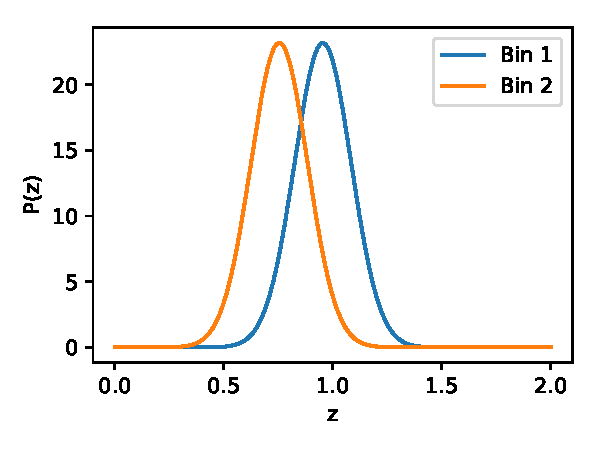
\includegraphics[width=0.6\textwidth]{./figures/pz.pdf}
        \caption{Galaxy distribution redshift bins.}
        \label{fig:pz}
      \end{figure}

      \begin{figure*}
        \centering
        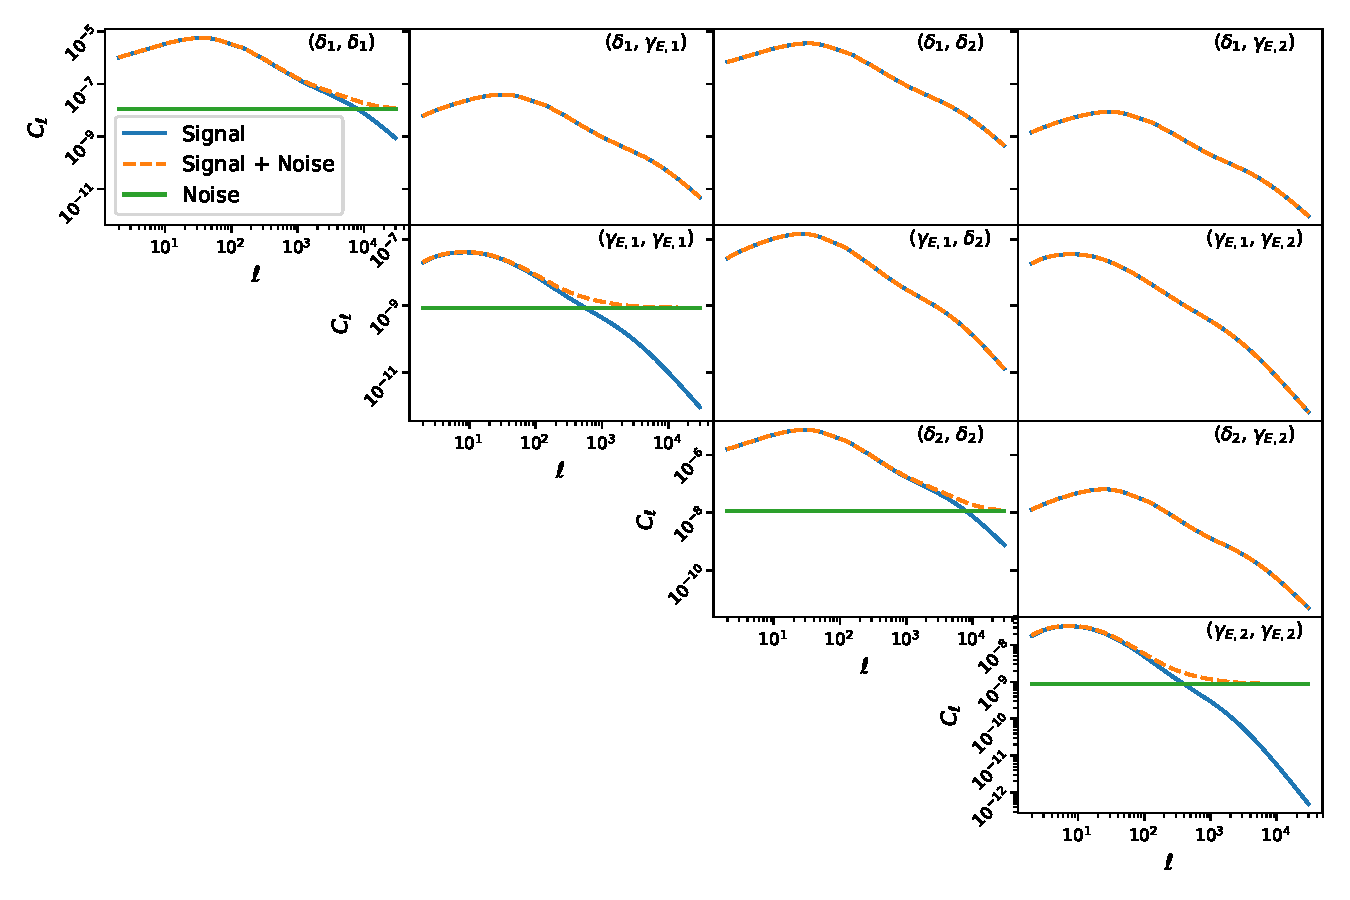
\includegraphics[width=\textwidth]{./figures/cls-sph-2b.pdf}
        \caption{Fiducial power spectra. We show only the $T$ and $E$ modes.}
        \label{fig:cl-2bins}
      \end{figure*}
      As we noted in Section~\ref{ssec:theory.pcl}, surveys are not able to observe all sky equally. Mathematically this means that the true random fields that fill the space will have a mask on top of them (Eq.~\ref{eq:mask}). This introduces mode coupling between different $\cl$ (Eq.~\ref{eq:M}) and highly complicates the expressions for the pseudo-$\cl$ covariance matrix of (see Section~\ref{ssec:theory.pcl} for the details). In order to prevent to overestimate the goodness of the NKA, we applied two different realist masks, which can be seen in Fig.~\ref{fig:mask}. Similar results were obtained using the same mask on both redshift bins.

      \begin{figure}
        \centering
        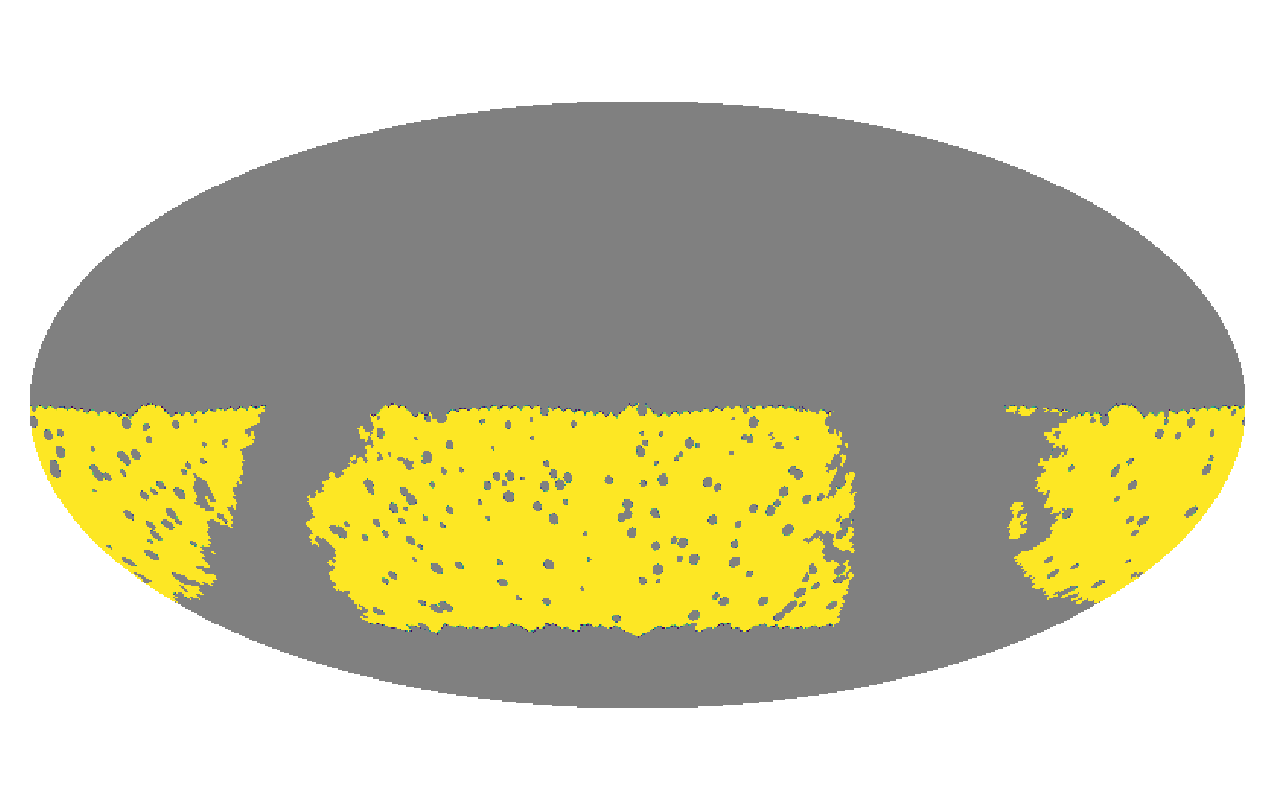
\includegraphics[width=0.45\textwidth]{./figures/mask-lss1.pdf}
        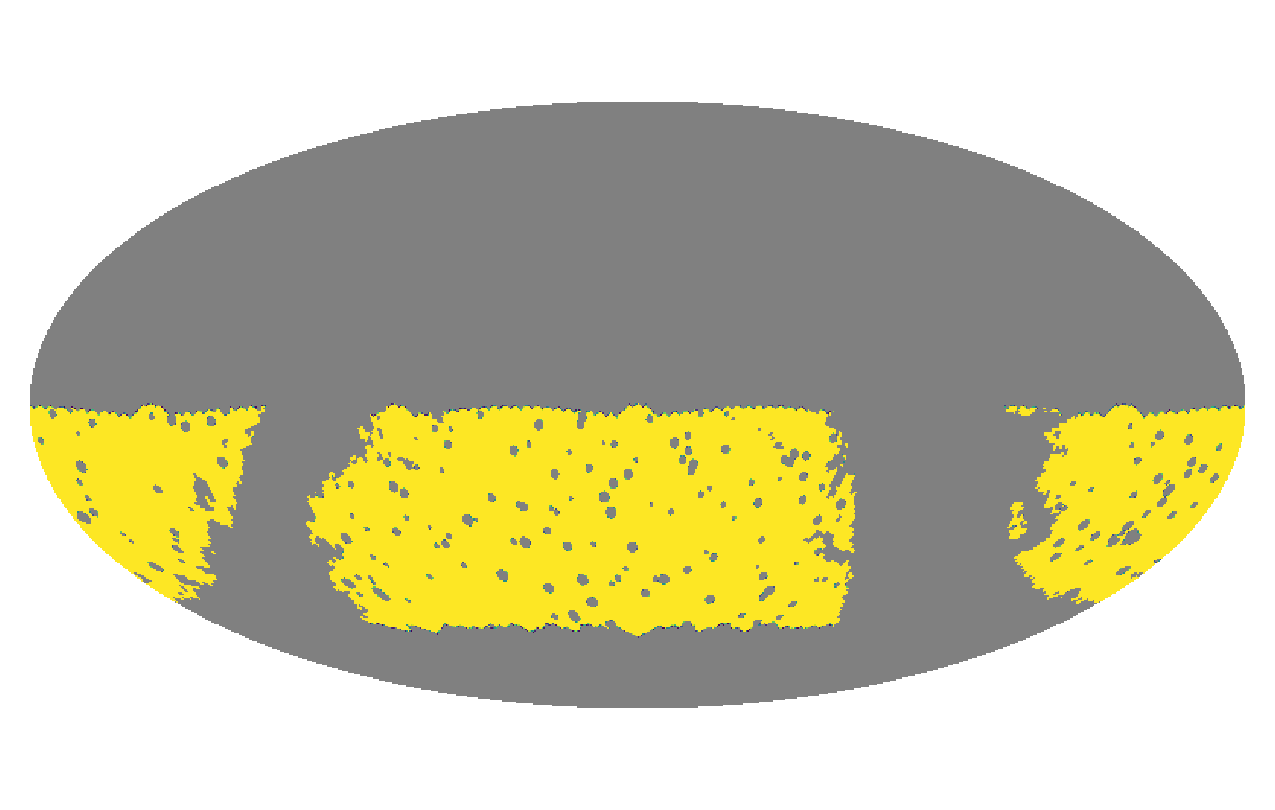
\includegraphics[width=0.45\textwidth]{./figures/mask-lss2.pdf}
        \caption{Sky mask used in our analysis} \label{fig:mask}
      \end{figure}
      The covariance matrices were obtained from 20000 simulations, for the band powers determined by the fraction of sky observed ($\Delta \lbpw = 1/\fsky$, $\fsky = \Pi_{\mbox{p}} \langle \mbox{masks} \rangle_{p}$, where $p$ stands for pixel). The highest accurate band power corresponds to $l_{\mbox{bpw}} = 1023$; i.e. $\sim 2 \times 512$, where 512 is the \todo{nside} of our maps. To work with the sky maps and masks we used \textit{HEALPix}\footnote{\url{https://healpix.jpl.nasa.gov/}}, whereas \textit{NaMaster}\footnote{\url{https://github.com/LSSTDESC/NaMaster}}~\cite{2018arXiv180909603A} was used for the computation of the pseudo-$\cl$ and the covariances. Our code is publicly available~\footnote{\url{https://github.com/damonge/PCLCovariance}}.


    \subsection{Visual inspection}\label{ssec:results.visual}
      In this section, we will present a qualitative analysis of the NKA covariance matrices. The idea is to identify what NKA is good able to reproduce accurately. We will focus here on some terms of the covariance matrix and the full correlation matrix.

      The NKA correctly reproduces the mask induced mode coupling, as well as the size of the covariances (see Fig.~\ref{fig:rows_1bin}) for the cases that do not include the $\gamma_B$-modes \todo{explain why this is expected}. It must be noted that the terms involving the $\gamma_E$-modes also give worse result that those with $\delta$, specially at large scales (low $\ell$). We will see, however, that they are small enough to not impact on the parameter estimation. The normalization chosen for Fig.~\ref{fig:rows_1bin} is that of the numerator of the naive covariance, which is given by
      \begin{equation}
        C(\cl^{ab}, \cl^{cd}) = \frac{\cl^{ac}\cl^{bd} + \cl^{ad}\cl^{bc}}{\fsky (2\ell + 1) \Delta\lbpw}\,,
        \label{eq:naive}
      \end{equation}
      where $\Delta \lbpw$ is the width of the binning of the $\ell$-band. This diagonal approximation is also unable to recover the correct size of the peaks in the covariance.

      \begin{figure}[htb]
        \centering
        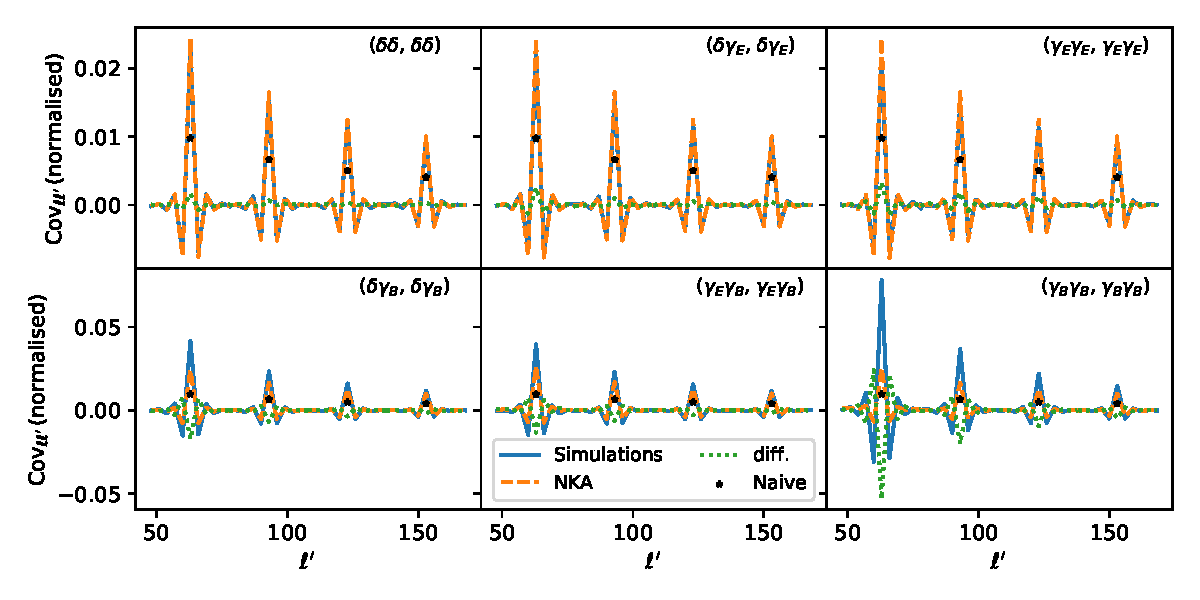
\includegraphics[width=\textwidth]{./figures/all_rows_sph_1bin.pdf}
        \caption{$\cl$ correlations for the different approximations and modes. It can be seen the mask induced coupling, which the NKA approximation is able to reproduce accurately.} \label{fig:rows_1bin}
      \end{figure}

      The difference of the full NKA and simulations' correlation matrices, which is a more general check, shows no structure in Fig.~\ref{fig:diff_corr_1bin}, except for the $\gamma_B$-modes. There is also some structure, at low $\ell$, in the $\gamma_E\gamma_E$ case. This results are coincident with previous analysis. What we call structure are systematic differences between the simulations and the NKA matrices. In contrast, those terms that are correctly recovered (i.e. the $\delta \delta$, $\delta \gamma_E$, $\gamma_E \gamma_E$ combinations), deviate from each other just by numerical issues, and are displayed as noisy regions.

      \begin{figure}[htb]
        \centering
        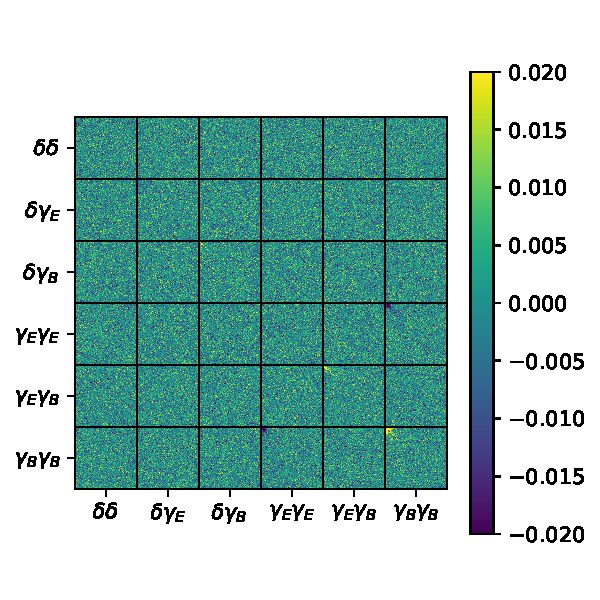
\includegraphics[width=0.6\textwidth]{./figures/sph_1bin_diff_corr.pdf}
        \caption{Correlation matrices difference between that of the simulations and the NKA. There is no structure except for the $\gamma_B$ modes and the $(\gamma_E\gamma_E, \gamma_E\gamma_E)$ case. In this case, it is only present at low scales and in a more mildly way.} \label{fig:diff_corr_1bin}
      \end{figure}

      More quantitatively, the NKA covariance matrix eigenvalues, for the observational interesting case $(\delta\delta-\delta\gamma_E-\gamma_E\gamma_E)$ deviate around 5\% from those of the simulations. 
      \begin{figure}[htb]
        \centering
        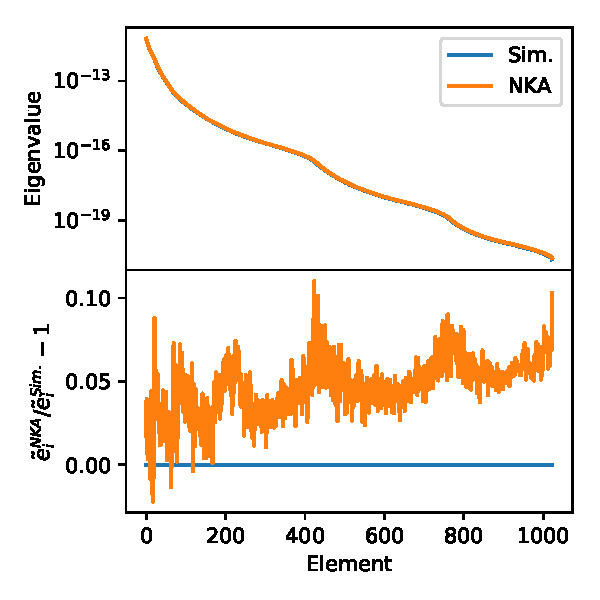
\includegraphics[width=0.6\textwidth]{./figures/run_sph_2b_NKA_TTTEEE_reldev_eigval_1stbin.pdf}
        \caption{Covariance matrix eigenvalues and the relative difference with respect to the eigenvalues from the simulations and NKA covariances.} \label{fig:eigv_1bin}
      \end{figure}

    \subsection{Quantitative checks}\label{ssec:results.quant}
      For a quantitative analysis of the covariance matrix and the analytical approximations, we computed the quantity 
      \begin{equation}
        (\cl - \langle \cl \rangle )C^{-1} (\cl - \langle \cl \rangle)\,, \label{eq:chi2-def}
      \end{equation}
      which, given the fact the simulations are drawn from Gaussian fields, should follow a $\chi^2$ distribution.

      The NKA works best for the $(\delta \delta, \delta, \delta)$ covariance. Involving $\gamma_E$ modes shift the distribution at lower $\chi^2$, but with the same overall shape. \todo{why is this expected?}. In Fig.~\ref{fig:chi2_1bin}, the distributions are shown. It is noticeable the good agreement of the naive spin-0 approximation with the more phsysical NKA. The simulations follow a $\chi^2$ distribution, as in the $(\delta \delta, \delta, \delta)$ case. As we mentioned, the more the $\gamma_E$ contributes, the more shifted the distribution is. However, in section \ref{ssec:results.cosmo} we will show this difference has no impact on the cosmological parameter estimation.

      \begin{figure}[htb]
        \centering
        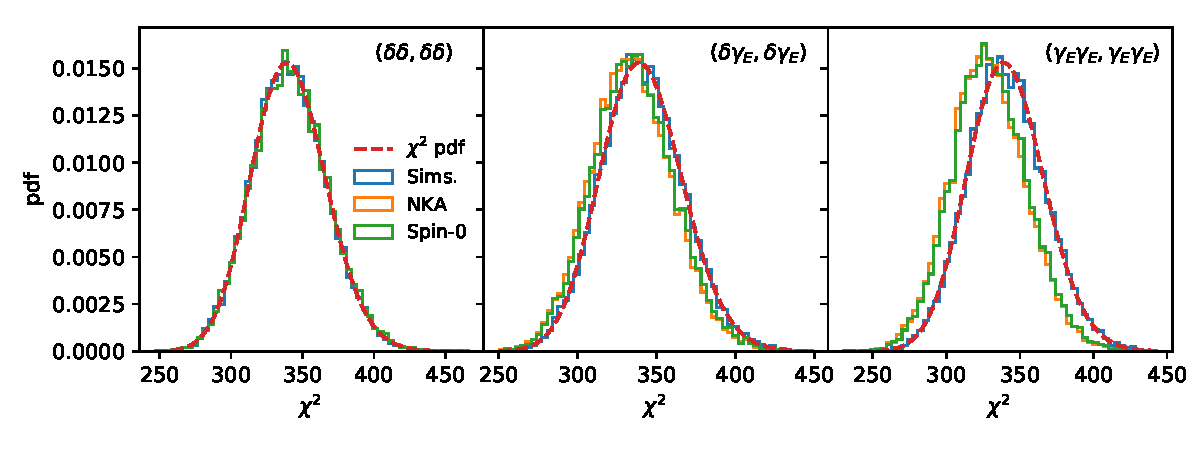
\includegraphics[width=\textwidth]{./figures/run_sph_2b_1stbin_chi2_TT_TE_EE.pdf}
        \caption{Plot $\chi^2$ TT-TT, TE-TE, EE-EE. \todo{Join them, sharey}} \label{fig:chi2_1bin}
      \end{figure}

      \todo{Talk about TT-TE-EE chi2?}

    \subsection{Contaminant deprojection}\label{ssec:results.deproj}
      The discussed results remain the same even in the presence of observational contaminants. In Fig.~\ref{fig:chi2_conts}, we show that the distributions drawn from simulations with and without contaminants are the same. The contaminants power spectrum was parametrized as follow
      \begin{equation}
        \clc = A (l + 1)^{\beta}\,.
        \label{eq:conts}
      \end{equation}
      In this equation, $A$ fixes the ration between the contaminant and signal power spectra at a certain scale. We chose $\clc/\clth = 0.1$ at $\ell=400$. In addition, $\beta$ was chosen randomly from a uniform distribution $U[-3,-1)$, for large-scale contaminants, and fixed to $\beta=0$, for small-scale contaminants. 

      \begin{figure}[htb]
        \captionsetup[subfigure]{width=0.40\textwidth}
        \centering
        \subfloat[$\chi^2$ distributions for the case with and without contaminants. We see they are perfectly removed.]{%
        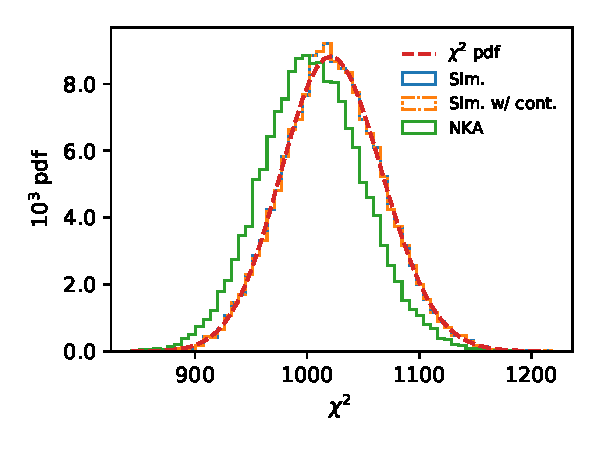
\includegraphics[width=0.49\textwidth]{./figures/contaminants_chi2.pdf}
        \label{fig:chi2_conts}%
        }
        \subfloat[$\cl^{\delta\delta}$ signal and contaminants power spectra. The limiting cases for the large-scale contaminants are given by $\beta=-1,\,-3$ in Eq.~\ref{eq:conts}, with $A$ fixed so that $\clc/\clth = 0.1$ at $\ell=400$.]{%
        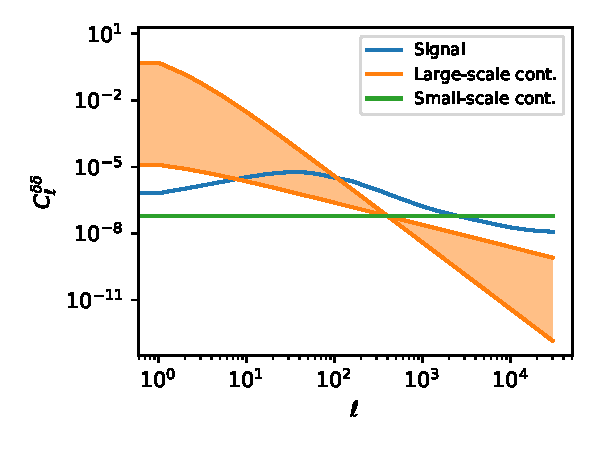
\includegraphics[width=0.49\textwidth]{./figures/contaminants_cl.pdf}
        \label{fig:conts}%
        }
        \caption{$\chi^2$ distributions from the simulations with contaminants and their power spectra.}
      \end{figure}

      In Fig.~\ref{fig:chi2_conts}) it is also shown the distribution obtained by the NKA covariance matrix for the joint case $(\delta\delta-\delta\gamma_E-\gamma_E\gamma_E)$. As we saw in previous section, the distribution is shifted respect to the $\chi^2$ distribution by the effect of the $\gamma_E$ modes.

    \subsection{Impact on parameter estimation}\label{ssec:results.cosmo}
      \begin{figure}[htb]
        \centering
        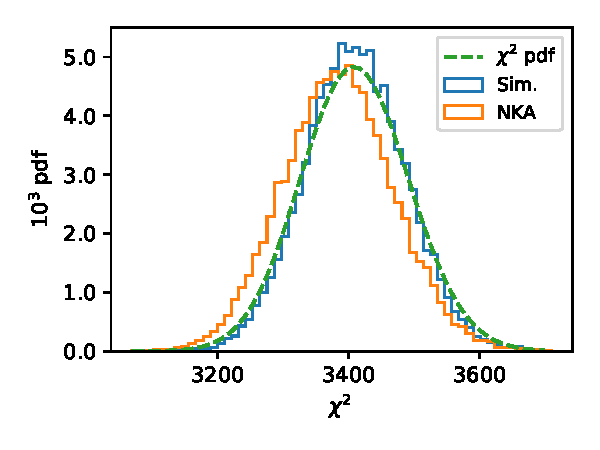
\includegraphics[width=0.6\textwidth]{./figures/run_sph_2b_same_mask_NKA_TTTEEE_Full_chi2.pdf}
        \caption{$\chi^2$ plot para 2 bines TT-TE-EE}
        \label{fig:chi2_2bins}
      \end{figure}

      \begin{figure}[htb]
        \centering
        \includegraphics[width=0.9\textwidth]{./figures/run_sph_2b_same_mask_NKA_diff_corr.pdf}
        \caption{Correlation difference between simulation's and NKA covariance matrices}
        \label{fig:corr_diff_2bins}
      \end{figure}

      \todo{Contours}

  \section{Discussion}\label{sec:discussion}


  \acknowledgments
  We would like to thank Eva-Maria Mueller for useful discussion. CGG is supported the Spanish grant BES-2016-077038, partially funded by the ESF and by AYA2015-67854-P from the Ministry of Industry, Science and Innovation of Spain and the FEDER funds. He was partially supported by a Balzan Fellowship while in Oxford. He would like to thank New College and the Department of Physics at Oxford for their hospitality. DA acknowledges support from STFC through an Ernest Rutherford Fellowship, grant reference ST/P004474/1.

%  \appendix


%\setlength{\bibhang}{2.0em}
%\setlength\labelwidth{0.0em}
  \bibliography{paper}
  
  
  \appendix
  \section{Flat sky}\label{app:flat}
    The NKA is even better in the flat sky regime. Using realist masks (Fig.~\ref{fig:mask_flat} we did the same analysis for flat sky. In this case, the NKA worked even for the $\gamma_B$ modes, being able to exactly recover the $\chi^2$ distributions (Fig.~\ref{fig:chi2_1bin_flat}).
    \begin{figure}[htb]
      \centering
      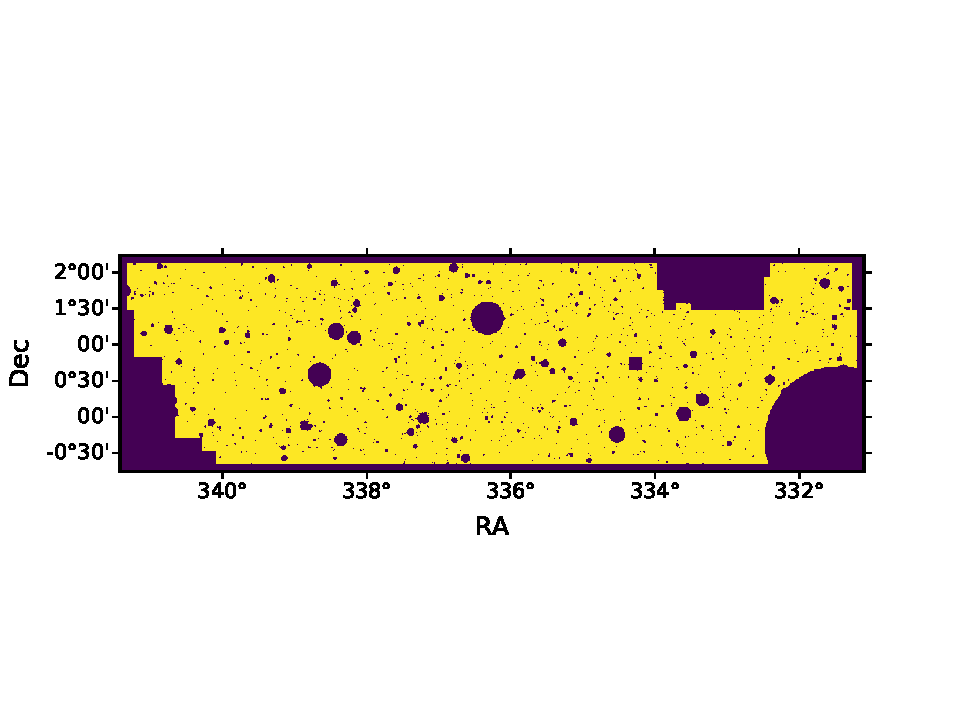
\includegraphics[width=0.6\textwidth]{./figures/mask-lss_flat1.pdf}
      \caption{Mask used for a flat-sky approximation in one of the redshift-bins} \label{fig:mask_flat}
    \end{figure}

    \begin{figure}[htb]
      \centering
      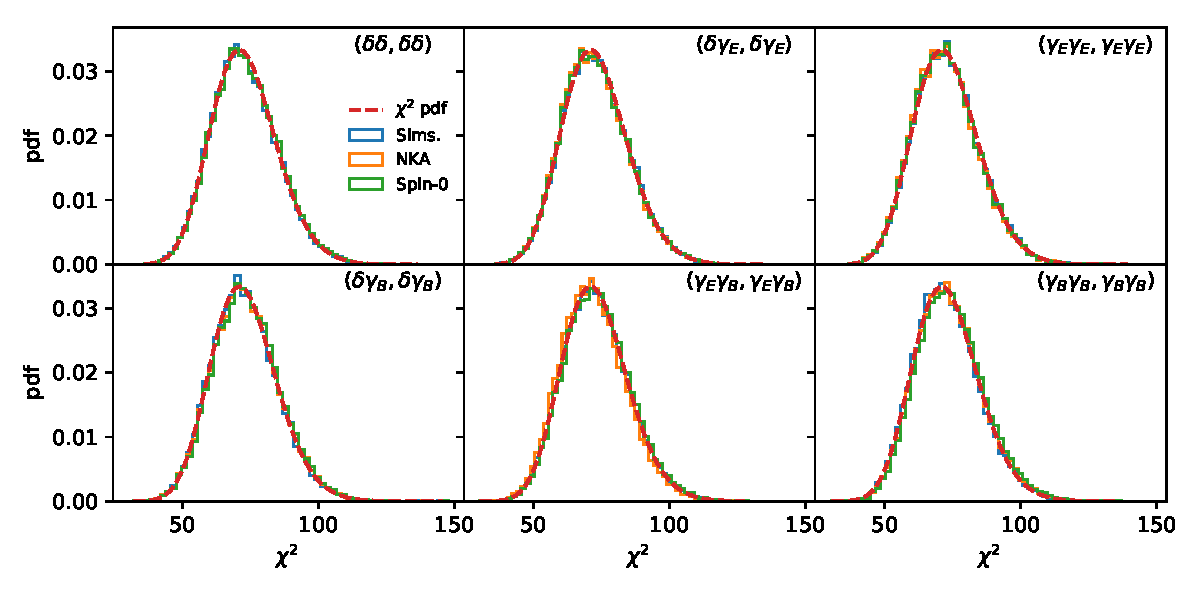
\includegraphics[width=\textwidth]{./figures/run_chi2_TT_TE_EE_TB_EB_BB.pdf}
      \caption{Plot chi2 TT-TT TE-TE, EE-EE}
      \label{fig:chi2_1bin_flat}
    \end{figure}

  \section{Software implementation}\label{app:namaster}
    \lipsum[4]

\end{document}
